\documentclass[tikz,border=2pt]{standalone}
\usepackage{amsmath,amssymb}
\usepackage{tikz}

\begin{document}
% A metric assigns a distance to every pair of points; the triangle inequality says the direct
% route x -> z is never longer than the detour through y.
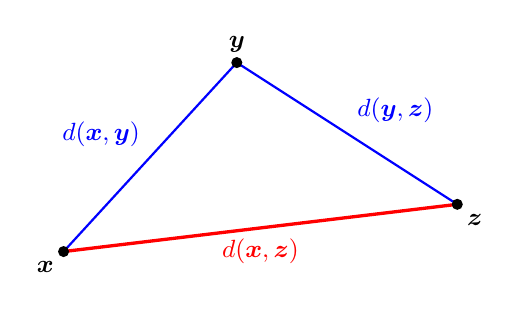
\begin{tikzpicture}[every node/.style={font=\small}]
	\coordinate (x) at (0,0);
	\coordinate (y) at (2.2,2.4);
	\coordinate (z) at (5,0.6);
	\draw[blue, thick] (x) -- (y) node[midway, above left] {$d(\boldsymbol{x},\boldsymbol{y})$};
	\draw[blue, thick] (y) -- (z) node[midway, above right] {$d(\boldsymbol{y},\boldsymbol{z})$};
	\draw[red, very thick] (x) -- (z) node[midway, below] {$d(\boldsymbol{x},\boldsymbol{z})$};
	\fill (x) circle (2pt) node[below left] {$\boldsymbol{x}$};
	\fill (y) circle (2pt) node[above] {$\boldsymbol{y}$};
	\fill (z) circle (2pt) node[below right] {$\boldsymbol{z}$};
\end{tikzpicture}
\end{document}
